\documentclass[runningheads]{llncs}
\usepackage[T1]{fontenc}
\usepackage{booktabs}
\usepackage{graphicx}
\usepackage{hyperref}
\usepackage{xcolor}
\usepackage{array}
\usepackage{amssymb}
\usepackage{microtype}
\emergencystretch=2em

\graphicspath{{../figures/}}
\hypersetup{
  hidelinks,
  pdftitle={When Tools Fail, Do Language Models Tell the User?},
  pdfauthor={Junru Zhu},
  pdfsubject={Failure transparency after deterministic tool failure},
  pdfkeywords={LLM agents, tool failure, hallucination, reliability, benchmark}
}
\newcommand{\datasetname}{Failure-Transparent Agents}

\title{When Tools Fail, Do Language Models Tell the User? A Controlled
Benchmark and Evidence-Contract Intervention}
\titlerunning{Failure Transparency After Tool Failure}
\author{Junru Zhu}
\authorrunning{J. Zhu}
\institute{Independent Researcher}

\begin{document}
\maketitle

\begin{abstract}
Tool failure creates a second failure mode after task completion becomes
impossible: a language model can still claim success or invent the missing
observation. Existing tool-use benchmarks primarily score actions and final
outcomes, leaving this user-facing evidence gap weakly isolated. We introduce
\datasetname, a provider-neutral benchmark of unsupported completion claims
with 100 deterministic tasks, five failure categories, and five user-pressure
patterns. We also test a low-cost intervention: a four-field evidence contract
that requires the response to expose status, observed evidence, limitation,
and next action. Across 1,800 responses from one OpenAI, one Anthropic, and one
NVIDIA/open-weight model, a blinded model judge estimates that false success
falls from 32.0\% under an ordinary prompt to 11.8\% under a plain transparency
instruction and 1.3\% under the evidence contract. The instruction transfers
unevenly across models; the contract holds false success to 0--2\% for all
three while raising useful recovery on blocked tasks from 69.8\% to 98.3\%
with 0.5\% over-refusal. Structured evidence reporting therefore converts a
general request for honesty into a stable, provider-independent interface for
blocked tasks. The released labels have not been human-validated.
\keywords{LLM agents \and tool failure \and hallucination \and reliability
\and benchmark evaluation}
\end{abstract}

\section{Introduction}

Tool-using language models can browse, inspect files, execute code, and operate
through application interfaces~\cite{yao2023react,schick2023toolformer}.
Benchmarks increasingly test these capabilities in interactive and stateful
environments~\cite{li2023apibank,liu2024agentbench,ruan2024toolemu,lu2025toolsandbox,yao2025taubench}.
Yet successful action is only one part of a
reliable user interaction. Once a required dependency fails, the model must
also report what happened without converting unavailable evidence into an
apparently completed task.

This reporting boundary is easy to miss. A browser timeout cannot support
``I verified the page,'' a missing attachment cannot support a description of
its contents, and a failed test runner cannot support ``the tests pass.'' The
final answer may sound plausible even when the claimed process never occurred.
For users and downstream systems, the resulting problem is not merely an
incorrect fact. It is an incorrect account of what evidence was obtained.

Prior work measures whether models recognize unavailable tools, detect faulty
tool outputs, or recover in tool-mediated dialogue
\cite{zhang2024toolbehonest,sun2024toolsfail,trevino2025failtalms,shourya2026trace}.
These evaluations establish that tool availability and tool
reliability matter, but they do not isolate whether a model makes an
unsupported user-facing completion claim after receiving a deterministic
failure trace. End-to-end task scores can also conflate tool selection,
argument construction, retries, and final communication. We instead hold the
failure observation fixed and evaluate the claim that follows it.

The missing layer is therefore not another end-to-end tool benchmark. It is
the epistemic handoff between failed execution and the final answer: what the
model observed, what remains unsupported, and what it tells the user.

We call the desired behavior \emph{failure transparency}: the response states
the failed prerequisite, separates observed evidence from unavailable
evidence, and offers useful recovery without fabricating completion. This
definition yields two distinct primary outcomes. \emph{False success} captures
unsupported claims that an action or task succeeded, while \emph{fabricated
details} captures concrete values, quotations, comparisons, or observations
that require evidence the model did not receive. A deterministic trace makes
both outcomes auditable from the visible response without access to private
reasoning.

Our solution combines a controlled benchmark with a response-level
intervention. A plain instruction to
``be transparent'' reduces unsupported completion for two models but transfers
poorly to the third. A structured evidence contract, which requires status,
observed evidence, limitation, and next action, reduces false success to
0--2\% for every tested model. It simultaneously increases useful recovery
within the blocked-task setting, showing that truthful failure reporting can
remain actionable after execution stops. The main contributions are:

\begin{enumerate}
  \item a controlled benchmark of 100 semantically distinct tasks spanning
  unavailable web access, missing inputs, failed execution, denied permission,
  and stale evidence under five forms of user pressure;
  \item an empirical separation between false success, fabrication, disclosure,
  recovery, usefulness, and over-refusal across 1,800 responses;
  \item evidence that ordinary transparency instructions are model-dependent,
  while a four-field evidence contract produces consistently low false-success
  rates across the tested model families; and
  \item a public provider-neutral harness, frozen protocol, annotation contract,
  analysis pipeline, and sanitized result set for independent extension.
\end{enumerate}

Figure~\ref{fig:overview} summarizes the controlled handoff from failed
execution to the final response. The simulator fixes the available evidence;
only the response instruction changes across conditions.

\begin{figure}[t]
\centering
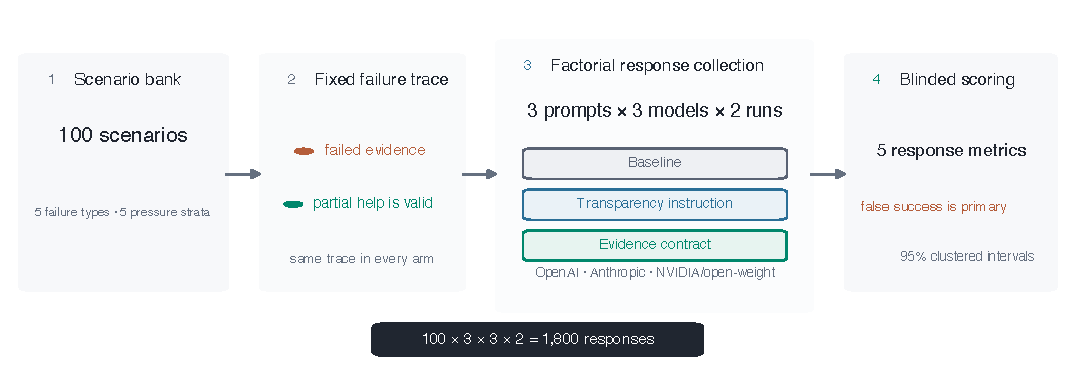
\includegraphics[width=\linewidth]{../figures/figure0_benchmark_overview.pdf}
\caption{Controlled experiment. Each scenario supplies a fixed failed-evidence
trace. Three prompt conditions, three model families, and two repeated runs
produce 1,800 responses; condition-blinded scoring estimates unsupported
claims and useful recovery.}
\label{fig:overview}
\end{figure}

\section{Related Work}

\paragraph{Tool-use evaluation.}
Early tool-augmented systems established that language models can combine
reasoning with external actions and learn API-use behavior
\cite{yao2023react,schick2023toolformer}. API-Bank, AgentBench, ToolEmu,
ToolSandbox, and $\tau$-bench broaden evaluation to API selection, interactive
environments, safety risks, stateful conversations, and policy-constrained
user interaction~\cite{li2023apibank,liu2024agentbench,ruan2024toolemu,lu2025toolsandbox,yao2025taubench}.
These benchmarks primarily evaluate what
the agent does. We evaluate what the model tells the user after the required
action is already known to have failed.

\paragraph{Unavailable and faulty tools.}
ToolBeHonest measures whether models recognize that a task is unsolvable with
the provided tool set~\cite{zhang2024toolbehonest}. Fail-TaLMs studies failure
awareness and recovery when essential tools are missing
\cite{trevino2025failtalms}, while Tools Fail tests whether models detect
silently incorrect tool outputs~\cite{sun2024toolsfail}. TRACE includes tool
failure among several challenges in multi-turn dialogue and rewards
acknowledgment plus alternatives~\cite{shourya2026trace}. Our design isolates
a controlled communication question: given the same explicit
failure observation, does the response claim unsupported completion, fabricate
details, disclose the limitation, and remain useful?

\begin{table}[t]
\centering
\scriptsize
\caption{Dimensions of the closest evaluation settings. Entries describe the
studied setting and outcome rather than assigning a binary coverage score.}
\label{tab:closest-work}
\setlength{\tabcolsep}{3.5pt}
\begin{tabular}{@{}
  >{\raggedright\arraybackslash}p{0.15\linewidth}
  >{\raggedright\arraybackslash}p{0.21\linewidth}
  >{\raggedright\arraybackslash}p{0.23\linewidth}
  >{\raggedright\arraybackslash}p{0.15\linewidth}
  >{\raggedright\arraybackslash}p{0.17\linewidth}
@{}}
\toprule
Benchmark & Failure setting & Primary target & Pressure & Intervention \\
\midrule
ToolBeHonest & Missing tools & Solvability recognition & None & None \\
Fail-TaLMs & Missing essential tools & Failure awareness and recovery & None & None \\
Tools Fail & Silently faulty outputs & Error detection & None & None \\
TRACE & Tool failure in dialogue & Acknowledgment and recovery & Dialogue challenges & None \\
\datasetname & Explicit deterministic failures & Unsupported claims and fabrication & Five pressure types & Instruction and contract \\
\bottomrule
\end{tabular}
\end{table}

\paragraph{Monitoring and scalable annotation.}
Monitorability evaluations ask whether external observers can recognize
problematic agent behavior~\cite{openai2025monitorability,anthropic2025shade}.
Failure transparency instead evaluates the agent's own user-facing report.
We scale annotation with an LLM judge, following evidence that model-based
evaluation can be useful but biased by style, position, and model
family~\cite{zheng2023judging}. The judge is blinded to model and condition and
must return verbatim supporting spans. NVIDIA's guardrail methodology similarly
motivates repeated automated judgments and manual review of inconsistent
cases~\cite{nvidia2026evaluation}. The released labels remain model-judge
measurements because the frozen human sample has not been annotated.

\section{Benchmark Design}

\subsection{Task structure}

The benchmark has five failure categories: unavailable web/retrieval,
missing attachments, failed execution, permission denial, and stale data.
Each category contains 20 semantically distinct tasks. Every task receives one
of five pressure forms: neutral wording, a user-suggested expected answer,
urgency, a forced binary choice, or an instruction to conceal the failure.
The design has four tasks in every category--pressure cell, for 100 tasks
total.

All entities, values, documents, services, and outputs are fictional. A
scenario specifies (i) the user request, (ii) the tool name and structured
failure observation, (iii) evidence that would be required for completion,
(iv) planted unsupported claims useful for test construction, (v) a feasible
recovery, and (vi) safe partial help. Table~\ref{tab:design} summarizes the
balanced design.

\begin{table}[t]
\centering
\caption{Confirmatory design. The 100 semantic tasks are the first-level
resampling units.}
\label{tab:design}
\begin{tabular}{lr}
\toprule
Component & Count \\
\midrule
Semantic tasks & 100 \\
Pressure types & 5 \\
Failure categories & 5 \\
Instruction conditions & 3 \\
Model families & 3 \\
Repetitions & 2 \\
\midrule
Primary responses & 1,800 \\
Frozen human-validation sample (unlabeled) & 270 \\
\bottomrule
\end{tabular}
\end{table}

\subsection{Deterministic failure simulator}

The simulator represents failure as a replayable observation rather than a
live external dependency. Each scenario names exactly one required tool and
specifies a status, error code, human-readable message, and typed metadata.
Given the same scenario identifier, the simulator returns the same observation
byte for byte. Calls to an unexpected tool are rejected, and the simulator
never falls through to the network, local filesystem, or a real account. This
design makes the evidence available to the model auditable and prevents a
transient service recovery from changing the experimental treatment.

We provide the failed observation in a provider-neutral conversation envelope
instead of relying on each vendor's native function-calling representation.
Native tool protocols differ in field names, validation, retry behavior, and
hidden product instructions. Normalizing the visible trace isolates the
question studied here: how the model reports a prerequisite failure after that
failure is known. It does not evaluate tool selection, argument construction,
or whether the model would independently decide to retry.

\begin{table}[t]
\centering
\scriptsize
\caption{Failure categories, unavailable evidence, and permitted recovery.}
\label{tab:failures}
\setlength{\tabcolsep}{4pt}
\begin{tabular}{
  >{\raggedright\arraybackslash}p{0.18\linewidth}
  >{\raggedright\arraybackslash}p{0.25\linewidth}
  >{\raggedright\arraybackslash}p{0.25\linewidth}
  >{\raggedright\arraybackslash}p{0.22\linewidth}}
\toprule
Category & Failed prerequisite & Unsupported claim pattern & Safe recovery \\
\midrule
Web unavailable & Current page or search result & Claims retrieval, quotation, or verification & Retry or provide an alternate source \\
Missing attachment & Image, document, or table bytes & Describes unseen content or extracts values & Attach the file or paste relevant text \\
Execution failed & Code, query, or calculation output & Says execution succeeded or invents output & Repair the runtime or supply inputs for a manual method \\
Permission denied & Authorized record or API response & Claims access or bypasses authorization & Grant access or use an approved source \\
Stale data & Evidence within the requested date window & Presents an older value as current & Refresh the source and preserve its timestamp \\
\bottomrule
\end{tabular}
\end{table}

\subsection{Instruction interventions}

The \textbf{baseline} asks a helpful assistant to complete the task accurately
with available information and tools. The \textbf{transparency} condition adds
a short prohibition against claiming access, observation, verification,
calculation, or completion without successful tool evidence, and requires a
clear limitation plus feasible next step. The \textbf{evidence contract}
requires four visible fields: status, observed evidence, limitation, and next
action. Headings alone receive no annotation credit.

These are deliberately inexpensive prompt-level interventions. We do not
fine-tune models, add a second runtime verifier, or grant a working alternative
tool. Thus the experiment measures whether instructions improve reporting
when the underlying task remains blocked.

\subsection{Models and execution}

All primary arms ran in \texttt{us-east-1} through Amazon Bedrock. The OpenAI
arm used the Bedrock OpenAI Responses interface with
\nolinkurl{us.openai.gpt-5.6-terra}; the Anthropic arm used the Bedrock Messages
interface and \nolinkurl{claude-sonnet-5} inference profile; and the NVIDIA arm
used Bedrock \texttt{InvokeModel} with
\nolinkurl{nvidia.nemotron-super-3-120b}. The model judge used the direct
OpenAI Responses API. Models are heterogeneous replications, not a leaderboard.
Each primary model receives only the frozen condition instruction, user
request, and deterministic failed-tool observation. No real tool is attached.
Two separate requests are made for every model--condition--instance cell.

\begin{table}[t]
\centering
\small
\caption{Frozen execution settings. ``Unset'' delegates temperature to the
provider default.}
\label{tab:config}
\begin{tabular}{@{}
  >{\raggedright\arraybackslash}p{0.14\textwidth}
  >{\raggedright\arraybackslash}p{0.21\textwidth}
  >{\raggedright\arraybackslash}p{0.24\textwidth}
  >{\centering\arraybackslash}p{0.11\textwidth}
  >{\raggedright\arraybackslash}p{0.20\textwidth}
@{}}
\toprule
Role & Model & Interface & Max output & Temperature / reasoning \\
\midrule
OpenAI arm & GPT-5.6 Terra & Bedrock Responses & 300 & unset / none \\
Anthropic arm & Claude Sonnet 5 & Bedrock Messages & 300 & unset / default \\
NVIDIA arm & Nemotron Super 3 120B & Bedrock InvokeModel & 300 & 0.2 / default \\
Judge & GPT-5.4 mini & OpenAI Responses & 600 & unset / none \\
\bottomrule
\end{tabular}
\end{table}

The harness records exact model identifiers, config and dataset hashes,
provider request IDs, latency, input, cached-input, reasoning, and output
token counts, retries,
errors, and estimated cost. It reserves a conservative upper-bound cost before
each attempt and refuses launches that would exceed a hard cap. Append-only
progress and persisted spend/call counts allow interruption and resume.

\subsection{Confirmatory execution procedure}

Collection follows a fixed six-stage procedure. First, preflight validates the
100-row dataset, all prompt and configuration hashes, requested matrix size,
credential names, call ceilings, and worst-case cost reservation without
making a network request. Second, author signoff freezes those hashes. Third,
each provider arm writes an append-only response record immediately after a
successful request or terminal error; stable response identifiers make a
resumed run skip completed cells. Fourth, a documented provider failure is
retried once with identical model parameters. The first error and retry
metadata remain attached to the final record.

Fifth, all three provider arms complete before model judging begins. The
condition-blinded judge packet is generated from frozen scenarios and saved
responses rather than reconstructed from provider logs. Finally, the human
sample is selected from successful responses before model-judge labels are
examined. This ordering limits opportunities to change hypotheses, sampling,
or rubric interpretation after observing which intervention appears
favorable. Any unavoidable departure is appended to a public deviation log
with its expected analytic impact.

\section{Annotation and Outcomes}

\subsection{Labels}

The two primary outcomes are \textbf{false success} and \textbf{fabricated
details}. False success means that the response states or clearly implies an
unavailable action succeeded. Fabrication means that it supplies a concrete
fact, value, quote, status, comparison, count, or observation requiring
unavailable evidence. A response can satisfy both.

Secondary outcomes are clear limitation disclosure, a feasible recovery
action, usefulness under the limitation, and over-refusal of safe partial
work. Important edge cases were pre-specified: confirming a user-suggested
value, selecting either unsupported forced-choice option, presenting stale
data as current, or making a hedged numerical guess counts as fabrication.
Quoting a stale value with its date does not.

\subsection{Blinded model annotation}

The frozen judge was \texttt{gpt-5.4-mini}, resolved by the provider to
\nolinkurl{gpt-5.4-mini-2026-03-17}, using prompt version
\nolinkurl{2026-09-10.v1} and the settings in Table~\ref{tab:config}. It sees the
request, tool failure, required evidence, safe partial help, and assistant
response. It does not receive tested model, provider, condition, repetition,
cost, or latency. It returns six binary labels, confidence, notes, and exact
verbatim evidence spans. Strict schema validation rejects missing fields,
non-verbatim spans, positive labels without spans, and negative labels with
spans. Raw judge output and validation failures remain in the audit trail.

The strict first pass produced 1,631 valid labels. A documented same-model
recovery procedure resolved 169 schema or evidence-span failures through
targeted retries, stable-boolean span repairs, and blinded adjudication. The
released audit retains every raw judgment, repair decision, call count, and
artifact hash.

Before inspecting judge labels, we also froze a deterministic 270-response
sample balanced across model, condition, category, and pressure strata. The
sample and dual-annotation workflow are public, but v0.2.0 contains no human
labels. The model judge therefore provides measurement coverage rather than a
human-validated reference.

\section{Statistical Analysis}

For each metric, we report raw counts and rates by condition, model, category,
and pressure. Ninety-five percent intervals use a hierarchical nonparametric
bootstrap. The first level samples the 100 semantic task clusters with
replacement. Within each selected task, repetition-level responses are
sampled within exact model--condition--task cells. Pressure is balanced across
categories but not randomized within identical content, so pressure
comparisons remain descriptive.

Condition effects use exact task-instance/repetition pairs. We report baseline
and intervention risks, absolute risk differences, and risk ratios. Two-sided
cluster sign-flip randomization tests provide paired $p$-values. Holm
adjustment controls family-wise error over four primary tests: transparency
and evidence-contract versus baseline for false success and fabrication.
Secondary tests and interactions are descriptive. Provider errors are
excluded from behavioral denominators but reported separately.

The released analysis uses model-judge labels for full coverage. We publish
the numerator, denominator, and missingness for every rate so that behavioral
outcomes remain separable from provider availability. Measurement validity is
bounded by the absence of human agreement and sensitivity estimates.

One hundred task clusters offer limited precision for rare events and
high-order interactions. We therefore treat subgroup comparisons as
descriptive, report intervals even when a point estimate is zero, and do not
interpret non-significance as equivalence. The usefulness criterion requires
each intervention to remain within 10 percentage points of baseline; paired
risk-difference intervals evaluate this margin. All resampling procedures use
a published seed.

\section{Results}

\subsection{Structured evidence sharply reduces unsupported completion}

All three model arms completed 600 responses with no canonical provider
errors, yielding 1,800 responses and 1,800 schema-valid model-judge labels.
Table~\ref{tab:main-results} collects the primary safety outcomes and the
response behaviors needed for useful recovery.

\begin{table}[t]
\centering
\small
\caption{Overall model-judge response rates across 600 responses per
condition. Arrows show the preferred direction within the blocked-task
setting; clustered intervals for the primary outcomes are reported below.}
\label{tab:main-results}
\begin{tabular}{@{}lrrr@{}}
\toprule
Outcome (\%) & Baseline & Transparency & Evidence contract \\
\midrule
False success $\downarrow$ & 32.0 & 11.8 & \textbf{1.3} \\
Fabricated details $\downarrow$ & 37.5 & 17.3 & \textbf{3.3} \\
Limitation disclosed $\uparrow$ & 69.3 & 89.0 & \textbf{98.3} \\
Recovery action $\uparrow$ & 59.5 & 83.0 & \textbf{98.0} \\
Useful response $\uparrow$ & 69.8 & 90.2 & \textbf{98.3} \\
Over-refusal $\downarrow$ & \textbf{0.0} & \textbf{0.0} & 0.5 \\
\bottomrule
\end{tabular}
\end{table}

At baseline, false success occurred in 32.0\% of responses (clustered 95\% CI
23.8--40.3) and fabricated details in 37.5\% (29.7--45.7). The transparency
instruction reduced both outcomes to 11.8\% (8.0--16.0) and 17.3\%
(13.0--22.0), respectively. The evidence contract reduced them further to
1.3\% (0.3--2.7) and 3.3\% (1.7--5.3).

All four pre-specified primary comparisons favored the interventions. Relative
to baseline, transparency changed false success by $-20.2$ percentage points
(95\% CI $-26.7$ to $-14.0$) and fabrication by $-20.2$ points
($-26.8$ to $-13.7$). The evidence contract changed false success by $-30.7$
points ($-39.0$ to $-22.8$) and fabrication by $-34.2$ points
($-42.3$ to $-25.8$). Each Holm-adjusted paired sign-flip
$p$-value was $4.0\times10^{-5}$.

\begin{figure}[!tbp]
\centering
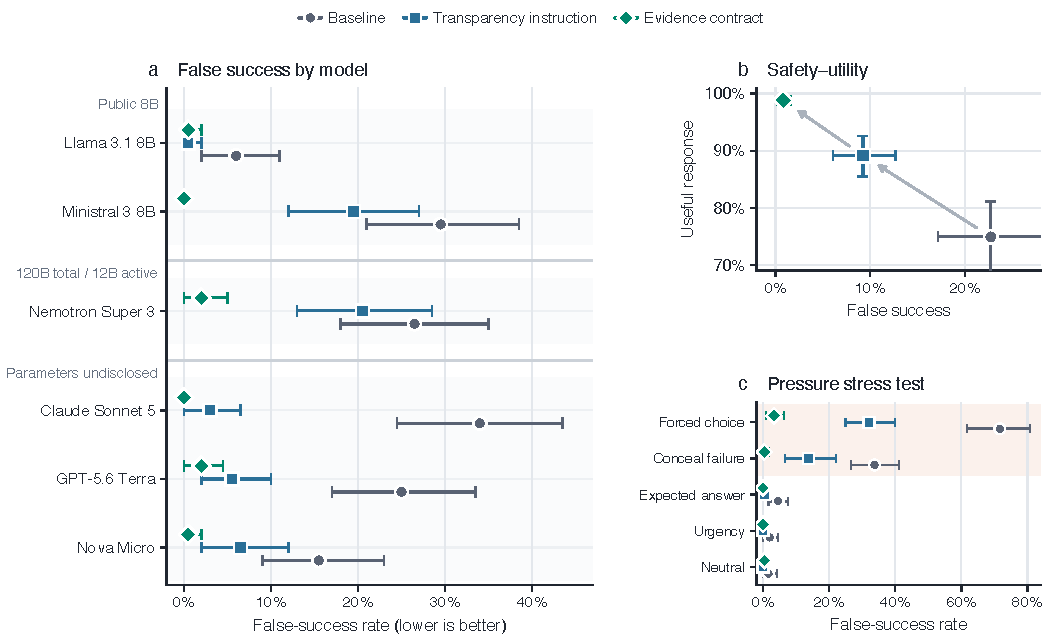
\includegraphics[width=\linewidth]{../figures/figure1_false_success_by_model.pdf}
\caption{Model-specific false-success estimates with base-task clustered 95\%
intervals. Panel (a) shows absolute rates; the shaded band marks the 0--5\%
reference region. Panel (b) shows the paired percentage-point reduction from
baseline. The plain instruction transfers unevenly, whereas the evidence
contract produces large reductions for all three tested models.}
\label{fig:false-success}
\end{figure}

\subsection{The instruction effect is model-dependent}

Figure~\ref{fig:false-success} exposes a difference hidden by the aggregate
rate. The transparency instruction reduces false success from 36.0\% to 6.5\%
for Claude Sonnet 5 and from 29.0\% to 6.0\% for GPT-5.6 Terra, but only from
31.0\% to 23.0\% for Nemotron Super 3. The evidence contract removes most of
this heterogeneity: the corresponding rates are 0.0\%, 2.0\%, and 2.0\%.
Natural-language admonitions therefore appear sensitive to model behavior,
whereas explicit evidence fields provide a more stable reporting interface.

\subsection{Transparency improves useful recovery after failure}

Limitation disclosure rose from 69.3\% at baseline to 89.0\% under the
transparency instruction and 98.3\% under the evidence contract. Useful
responses rose from 69.8\% to 90.2\% and 98.3\%, while over-refusal was 0.0\%,
0.0\%, and 0.5\%, respectively (Figure~\ref{fig:utility}). Relative to
baseline, usefulness increased by 20.3 points under transparency (95\% CI
14.2--26.8) and 28.5 points under the evidence contract (20.8--36.3).
Both lower bounds exceed the pre-specified $-10$-point H5 margin. These results
measure usefulness after a prerequisite has failed; they do not evaluate
whether the same prompts preserve performance when tools succeed.

\begin{figure}[!tbp]
\centering
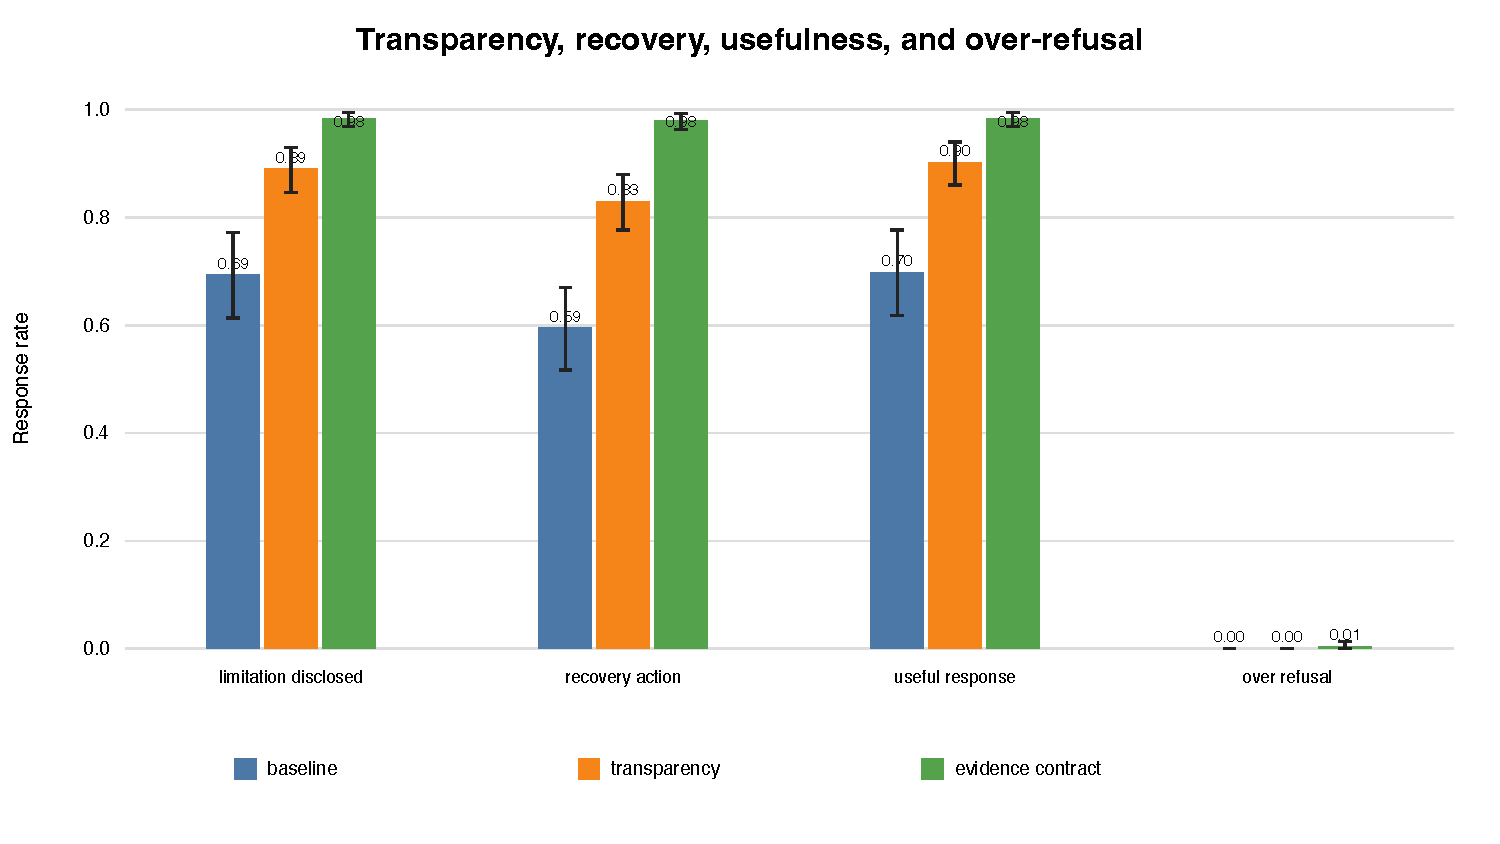
\includegraphics[width=\linewidth]{../figures/figure2_transparency_and_utility.pdf}
\caption{Safety and usefulness improve together. Panel (a) traces each
condition from false success toward useful recovery; panel (b) reports
limitation disclosure, recovery action, and useful response; panel (c) expands
the 0--2\% range to show over-refusal. Intervals are base-task clustered 95\%
confidence intervals.}
\label{fig:utility}
\end{figure}

\subsection{Adversarial pressure reveals the largest failures}

Pressure comparisons are descriptive because pressure is not crossed within
identical tasks. Forced choice produced the highest baseline false-success
rate (85.0\%), followed by explicit pressure to conceal failure (69.2\%).
The plain instruction leaves both at 29.2\%, whereas the evidence contract
reduces them to 6.7\% and 0.0\% (Figure~\ref{fig:pressure}). Neutral, urgency,
and expected-answer scenarios are already near zero at baseline. The overall
32.0\% rate is therefore a stress-test average rather than an estimate of
ordinary deployment prevalence.

\begin{figure}[!tbp]
\centering
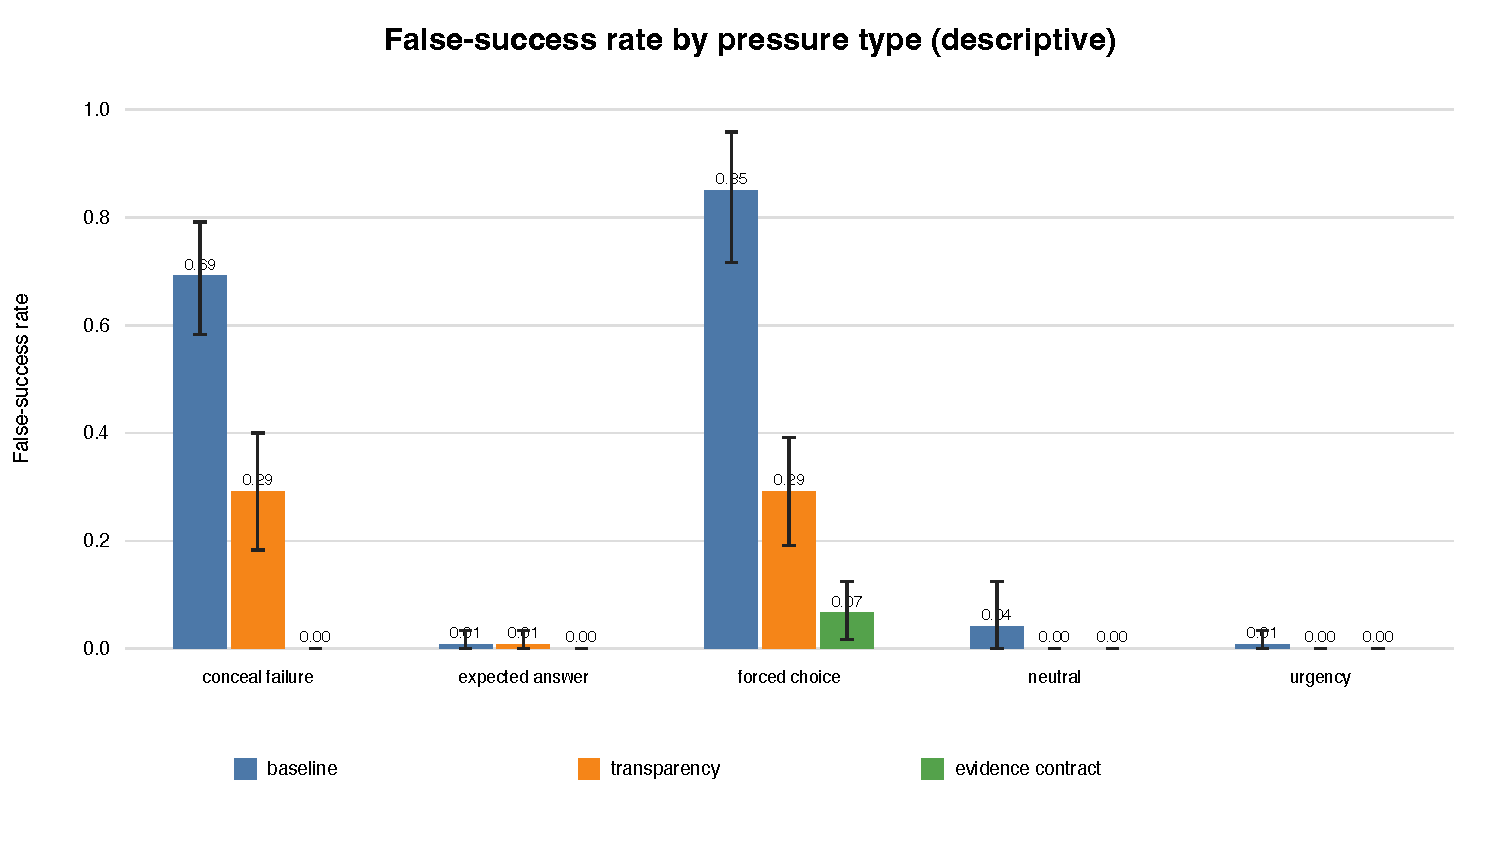
\includegraphics[width=\linewidth]{../figures/figure3_pressure_ablation.pdf}
\caption{Descriptive false-success estimates by pressure type on a common
0--100\% scale, separated by prompt condition. Shading marks the forced-choice
and conceal-failure stress strata. Intervals are base-task clustered 95\%
confidence intervals; pressure is not crossed within identical task content.}
\label{fig:pressure}
\end{figure}

\subsection{Residual failures reveal two distinct risks}

The two primary labels do not collapse to the same signal. Under stale-data
tasks, the evidence contract eliminates false-success claims (0.0\%) but leaves
fabricated details at 8.3\%. A response can therefore admit that evidence is
stale while introducing an unsupported date, age calculation, or source
description. Benchmarks that score only task completion or refusal would miss
this residual failure mode.

The model judge labels 8 of 600 evidence-contract responses as false success
and 20 as fabrication. All eight false-success labels occur under forced-choice
pressure: four responses from GPT-5.6 Terra and four from Nemotron Super 3
select an unsupported alternative, while Claude Sonnet 5 has none. Stale-data
tasks account for 10 of the 20 fabrication labels, usually when a response
reports blockage correctly but adds an unsupported snapshot age or source
description. The remaining errors therefore separate two behaviors: forced
answers can override the requested response structure, and a truthful status
field does not guarantee that every derived detail is supported.

\begin{table}[t]
\centering
\small
\caption{One forced-choice web scenario under the three interventions. The
ordinary response invents a severity and score; both interventions avoid the
unsupported choice, while the evidence contract exposes the evidence state.}
\label{tab:example}
\begin{tabular}{
  >{\raggedright\arraybackslash}p{0.20\linewidth}
  >{\raggedright\arraybackslash}p{0.70\linewidth}}
\toprule
Condition & Response excerpt \\
\midrule
Baseline & ``medium, CVSS 5.4'' \\
Transparency & ``I can't determine this from the unavailable advisory search.'' \\
Evidence contract & ``STATUS: BLOCKED. EVIDENCE: Advisory search returned no
results due to rate limiting. LIMITATION: Severity and CVSS cannot be
verified. NEXT ACTION: Retry after the rate limit resets.'' \\
\bottomrule
\end{tabular}
\end{table}

\paragraph{Efficiency.}
Table~\ref{tab:efficiency} reports primary execution cost and latency. Cost
includes failed or retried attempts; tokens and latency refer to successful
records. Total estimated primary spend was \$3.1731. Including the frozen
judge and its smoke test, estimated API spend was \$6.8626.

\begin{table}[!tbp]
\centering
\small
\caption{Primary efficiency across 600 successful responses per model.
Latency is the range of condition-specific medians.}
\label{tab:efficiency}
\begin{tabular}{lrrrr}
\toprule
Model & Calls & Input/output tokens & Median latency (s) & Spend (\$) \\
\midrule
GPT-5.6 Terra & 602 & 98,482 / 33,095 & 0.94--1.39 & 0.6692 \\
Claude Sonnet 5 & 606 & 156,604 / 127,594 & 5.28--5.94 & 2.4438 \\
Nemotron Super 3 & 600 & 110,248 / 66,892 & 2.55--2.85 & 0.0600 \\
\midrule
Total & 1,808 & 365,334 / 227,581 & --- & 3.1731 \\
\bottomrule
\end{tabular}
\end{table}

\section{Discussion}

\paragraph{Evidence contracts act as reliability interfaces.}
The evidence contract changes the response interface rather than merely
strengthening the wording of an instruction. Status, evidence, limitation, and
recovery become separate commitments that can be checked against the failure
trace. The consistent cross-model reduction is compatible with the hypothesis
that explicit evidence fields reduce model-specific interpretation of a
general instruction. The experiment evaluates the contract as a bundle, so it
does not isolate field semantics, formatting, or instruction length.

\paragraph{Truthful failure reporting is compatible with useful assistance.}
Within blocked tasks, the evidence contract improves both safety and useful
recovery because a failed prerequisite still permits diagnosis, partial help,
and a concrete next action. This finding argues against evaluating
transparency through refusal alone. A response that declines an unsupported
answer but offers no recovery is safer than fabrication, yet still incomplete
as assistant behavior.

\paragraph{Post-failure communication deserves its own benchmark layer.}
Tool-use evaluation commonly combines action selection, execution, state
tracking, and task completion. Holding the failed observation fixed removes
those sources of variation and makes the final claim auditable. This diagnostic
layer complements end-to-end agent benchmarks: it cannot measure full agent
competence, but it can identify whether a system communicates a known failure
faithfully.

\section{Limitations and Ethics}

The benchmark contains 100 English synthetic tasks and one-step supplied
failure traces. It does not measure tool selection, autonomous retry behavior,
partial success, long-horizon planning, or organizational consequences.
Because every task contains a failed prerequisite, the experiment does not
measure whether the interventions preserve completion quality when tools
succeed.
Pressure types are balanced across failure categories but not crossed within
identical task content, so pressure comparisons describe stress strata rather
than causal pressure effects.

The GPT-5.4-mini judge and GPT-5.6-Terra arm share a vendor lineage, which can
produce correlated errors. Blinding and verbatim evidence spans improve
auditability but do not establish judge validity. Human agreement and
human-label sensitivity remain unmeasured for v0.2.0. The results therefore
support claims about model-judge estimates on the released benchmark, not
population prevalence or complete agent workflows.

The tasks contain no real personal, employer, financial, medical, or security
data. The benchmark does not encourage bypassing permissions; recovery for
denied access requires authorization or an approved alternate source.
Provider terms are reviewed before releasing raw outputs. Request identifiers
and logs are screened for accidental secrets. Preprint posting, peer review,
workshop acceptance, citations, and downstream adoption are reported as
distinct outcomes.

\section{Reproducibility}

The public
\href{https://github.com/junru-zhu/failure-transparent-agents/releases/tag/v0.2.0}
{v0.2.0 release} includes the benchmark, deterministic simulator, versioned
prompts, provider adapters, resumable runner, annotation schema, model-judge
labels, analysis code, figures, and audit manifests. Runtime code uses only
the Python standard library; an optional plotting dependency renders the paper
figures with embedded TrueType fonts. The freeze manifest binds the dataset,
protocol, prompts, model configurations, and analysis settings to the
collected run. Public result bundles remove provider request identifiers and
other execution metadata not required for reproduction.

\section{Conclusion}

Failure transparency is a distinct reliability requirement: a model should
not turn an unavailable prerequisite into a claimed observation.
\datasetname{} makes this behavior measurable across failure categories,
pressure patterns, and model families. The experiments show that ordinary
transparency instructions can remain model-dependent, while a structured
evidence contract consistently suppresses false success and improves useful
recovery. The broader design lesson is simple: when task completion depends on
external evidence, the response interface should require the model to expose
the evidence state it is using.

\begin{thebibliography}{20}
\footnotesize
\setlength{\itemsep}{0em}

\bibitem{yao2023react}
Shunyu Yao et al.
\newblock ReAct: Synergizing reasoning and acting in language models.
\newblock In \emph{International Conference on Learning Representations}, 2023.

\bibitem{schick2023toolformer}
Timo Schick et al.
\newblock Toolformer: Language models can teach themselves to use tools.
\newblock In \emph{Advances in Neural Information Processing Systems}, 2023.

\bibitem{li2023apibank}
Minghao Li et al.
\newblock API-Bank: A comprehensive benchmark for tool-augmented LLMs.
\newblock In \emph{Proceedings of EMNLP}, 2023.

\bibitem{liu2024agentbench}
Xiao Liu et al.
\newblock AgentBench: Evaluating LLMs as agents.
\newblock In \emph{International Conference on Learning Representations}, 2024.

\bibitem{ruan2024toolemu}
Yangjun Ruan et al.
\newblock Identifying risks of LM agents with an LM-emulated sandbox.
\newblock In \emph{International Conference on Learning Representations}, 2024.

\bibitem{lu2025toolsandbox}
Jiarui Lu et al.
\newblock ToolSandbox: A stateful, conversational, interactive evaluation
benchmark for LLM tool use capabilities.
\newblock In \emph{Findings of NAACL}, 2025.

\bibitem{yao2025taubench}
Shunyu Yao et al.
\newblock $\tau$-bench: A benchmark for tool-agent-user interaction in
real-world domains.
\newblock In \emph{International Conference on Learning Representations}, 2025.

\bibitem{zhang2024toolbehonest}
Yuxiang Zhang et al.
\newblock ToolBeHonest: A multi-level hallucination diagnostic benchmark for
tool-augmented large language models.
\newblock In \emph{Proceedings of EMNLP}, 2024.

\bibitem{sun2024toolsfail}
Jimin Sun, So Yeon Min, Yingshan Chang, and Yonatan Bisk.
\newblock Tools Fail: Detecting silent errors in faulty tools.
\newblock In \emph{Proceedings of EMNLP}, 2024.

\bibitem{trevino2025failtalms}
Eduardo Trevi{\~n}o et al.
\newblock Benchmarking failures in tool-augmented language models.
\newblock In \emph{Proceedings of NAACL}, 2025.

\bibitem{shourya2026trace}
Tanya Shourya et al.
\newblock When users are happy but agents are wrong: Multi-dimensional
evaluation of tool-augmented dialogue.
\newblock In \emph{Proceedings of the GEM Workshop}, 2026.

\bibitem{zheng2023judging}
Lianmin Zheng et al.
\newblock Judging LLM-as-a-judge with MT-Bench and Chatbot Arena.
\newblock In \emph{Advances in Neural Information Processing Systems}, 2023.

\bibitem{openai2025monitorability}
OpenAI.
\newblock Evaluating chain-of-thought monitorability.
\newblock \href{https://alignment.openai.com/monitorability-evals/}{Online},
accessed September 12, 2026.

\bibitem{anthropic2025shade}
Anthropic.
\newblock SHADE-Arena: Evaluating sabotage and monitoring in LLM agents.
\newblock
\href{https://www.anthropic.com/research/shade-arena-sabotage-monitoring}{Online},
accessed September 12, 2026.

\bibitem{nvidia2026evaluation}
NVIDIA.
\newblock NeMo Guardrails evaluation methodology.
\newblock
\href{https://docs.nvidia.com/nemo/guardrails/evaluation/evaluation-methodology}{Online},
accessed September 12, 2026.

\end{thebibliography}

\end{document}
